\chapter{绪论}

\section{研究背景和意义}

进入二十一世纪以来,人们表示和传递信息的媒介从文本、声音扩展到了图像、视频。如今视频已经成为人们生产和生活中不可缺少的部分。另一方面,在计算机技术和通信技术的推动下,人们对网络的依赖和要求也越来越高。
智能手机、平板电脑等移动设备的普及,Wi-Fi、4G等无线网络的覆盖,让人们能够随时随地访问互联网。这样的环境催生并促进了一项技术的蓬勃发展,这就是视频流媒体。

视频流媒体简单来说就是通过网络在线播放视频。所谓流媒体,是指音视频等多媒体数据通过网络以连续稳定的流的形式传输到客户端的一系列技术、协议和方法的总称。在视频流媒体中,视频数据从服务器连续不断地传输到客户端,客户端可以一边接收一边播放,无需等待整个文件发送完毕。与下载方式相比,这种采用流式传输的视频播放具有显著的优点\supercite{Li2002},包括:1)启动延迟大大缩短,用户可以在等待几秒或十几秒的缓冲后就立即开始观看;2)视频数据不在客户端长时间驻留,不仅节省了用户存储空间,也一定程度上避免了内容版权保护问题;3)支持数据的实时生成和获取,大大扩展了视频应用场景的范围。正是由于其优秀的特性,视频流媒体得到了广泛的应用,逐渐成为人们消费视频内容的主要形式\supercite{Chen2013}。

视频流媒体应用按照其对实时性要求的不同可以分为点播和直播两大类。在点播应用中,内容提供商将预先制作好的视频放在服务器上,并发布内容的描述信息和链接,用户选择自己感兴趣的内容请求播放相应的视频。典型的例子是在线视频网站,如国外的YouTube\footnote{https://www.youtube.com/}、Netflix\footnote{https://www.netflix.com/},国内的优酷\footnote{http://www.youku.com/}、乐视\footnote{http://www.le.com/}等。大多在线教育网站如Coursera\footnote{https://www.coursera.org/}、网易公开课\footnote{http://open.163.com/}等也属于视频点播类应用。在直播应用中,视频数据则是通过现场录制实时生成的,上传到流媒体服务器之后再即时分发给观看者,具有很强的时效性。这类应用包括现在互联网上正兴起的秀场、游戏、生活类直播软件,以及已经很成熟的远程监控、视频会议等等。直播应用往往也会把实时事件的内容存储起来,后续以点播的形式继续提供。

网络条件的改善,采集与播放设备的普及,使得视频流媒体应用进入了一个高速增长的时期。根据Cisco的一项预测\footnote{http://www.cisco.com/c/en/us/solutions/collateral/service-provider/ip-ngn-ip-next-generation-network/white\_paper\_c11-481360.html},从2014年到2019年,视频流量在所有互联网流量中的占比将从64\%上升至80\%。路透社的一篇报道\footnote{http://www.reuters.com/article/us-internet-consumers-cisco-systems-idUSKBN0EL15E20140610}指出,在美国这一比例在2018年即将达到83\%。可见,视频流媒体正迎来一个高峰期。

在前所未有的机遇同时,视频流媒体也面临着网络异构和带宽波动所带来的严峻挑战。虽然有学者在探索下一代网络架构\supercite{Egilmez2014,Li2014,Xue2015},但现在传统的互联网架构仍将长期占据绝对主流地位。从当前的网络构成来看,既存在几百kb/s速度的拨号或3G上网,又有几十Mb/s速度的局域网或光纤接入,而且随着移动通信网与Internet的融合,无线与有线网络的混联,网络异构性更加明显。视频流媒体的终端用户可能处于不同的网络中(例如有线网,Wi-Fi,蜂窝移动网络等),甚至有可能在观看视频的过程中从一种网络切换到到另一种网络(典型的例子是手机用户在Wi-Fi和4G网络之间的切换)。即使是在同一网络环境中,视频传输可用的带宽也会因为网络拥堵情况的变化而不断波动。

在这样的实际条件下,如果视频流媒体系统以恒定的速率传输数据,将很难或者不可能会给用户带来最好的视频观看体验。举例来说,如果设置一个较低的码率,则对应的视频质量不高,达不到带宽充足用户的满意度;而如果设置较高的码率,则对于低带宽的用户或者在带宽波动较大的情况下,可能会导致视频无法流畅播放。因此,为应对这一挑战,视频流媒体系统需要能够根据不同的网络条件自动调整所发送视频的码率,以适应带宽的变化。换句话说,视频流媒体需要具备自适应性。

考虑到视频流媒体的广泛应用,通过加入自适应性来进一步改善视频流媒体服务质量,具有重要的现实意义。自适应视频流媒体的研究既受到了工业界的普遍关注,也成为了学术界的一大热点。

\section{研究框架和问题}

自适应视频流媒体的研究属于视频流媒体研究领域的一个子集。视频流媒体是视频与流媒体的结合,因此这个领域的研究也涉及包括编码和传输在内的多个方面。如图\ref{fig:research-framework}所示,视频流媒体的研究可以从系统模块的角度分为以下几个部分:

\begin{itemize}
	\item 数据源端的研究,一方面是进行高效的压缩编码,以尽可能少的数据表示尽可能高的视频质量;另一方面是提供具备灵活性的码流,支持码率的变化甚至考虑容错,等等。
	\item 传输过程的研究,即如何又快又好地将视频数据送给用户,包括改善网络状况以提高传输的吞吐量和可靠性,合理公平地利用带宽资源,根据带宽情况自适应地调整传输速率等。
	\item 客户终端的研究,即优化用户设备收到视频码流之后的播放阶段,包括如何快速解码,进行一些画质增强等后处理过程从而更好地显示,等等。
\end{itemize}

\begin{figure}[t]
	\centering
	\vspace{10pt}
	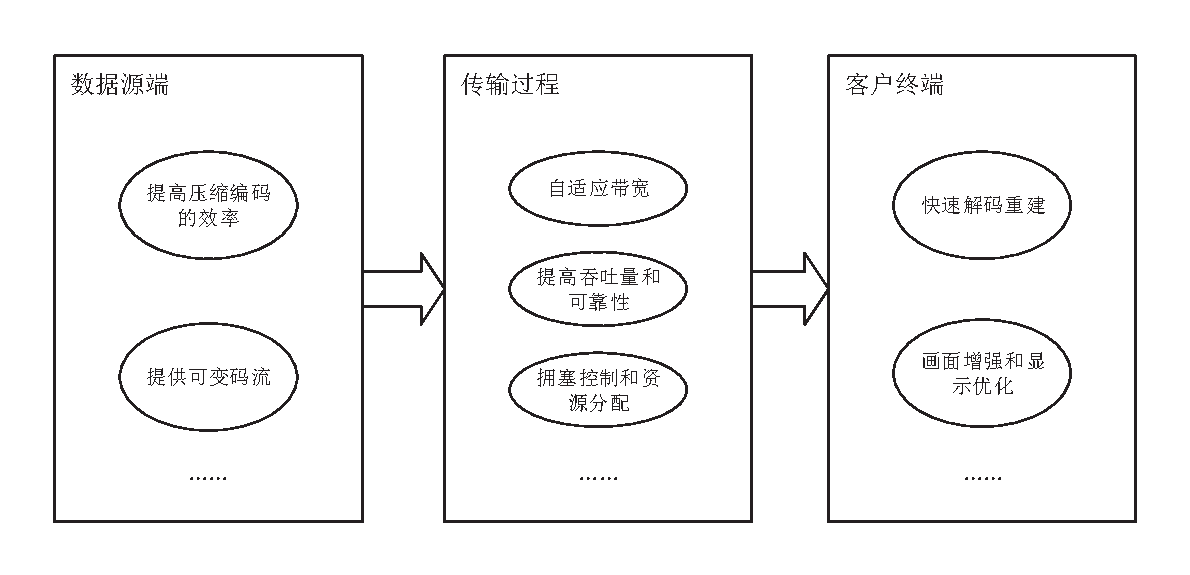
\includegraphics[width = 1.0\linewidth]{eps/research-framework}
	\caption{视频流媒体研究框架 \label{fig:research-framework}}
\end{figure}

\vspace{10pt}
在这一研究框架中,自适应视频流媒体主要涉及的是数据源端提供可变码率、传输过程中自动适应带宽这两个方面。虽然其他方面的研究工作,例如对编码效率的提升、对网络架构和协议的改进、在用户终端的解码优化等,也非常重要,但本文主要关注的是上述与自适应性相关的两个方面。

在视频流媒体系统中支持视频码率的可变性通常有两种选择。第一种选择是采取多码流的方法。多码流方法的原理很简单,就是预先编好不同码率的多个码流存放在服务器上,根据网络情况选取其中合适的一个进行传送。近年来兴起的HTTP动态自适应流媒体(Dynamic Adaptive Streaming over HTTP,  DASH)\supercite{Sodagar2011}就属于这类方法。如图\ref{fig:DASH}所示,DASH系统在服务器端提供不同码率的多个码流切片,客户端通过HTTP协议拉取数据,在某个时间段内可以选择性地接收这几个码流中任何一个的切片,通过在多个码流之间切换来更改码率以适应带宽波动。此外,有的系统会在服务器上将预先编好的一个高码率码流实时转码成不同低码率的码流,这本质上也属于多码流的方法。

第二种选择是采用可伸缩视频编码\supercite{SVC-Overview}技术。作为国际视频编码标准H.264/AVC\supercite{H.264}的扩展之一,可伸缩视频编码的初衷就是在单个码流中加入伸缩性的支持,使其码率和视频质量能够根据需要改变。可伸缩视频码流中的数据被划分为基本层和增强层数据包,可以从中丢弃一部分增强层数据包而截取出一个子流,以牺牲视频质量的方式来降低码率。因此,用它来实现码率可变性正符合其设计目的。

\begin{figure}[t]
	\centering
	\vspace{10pt}
	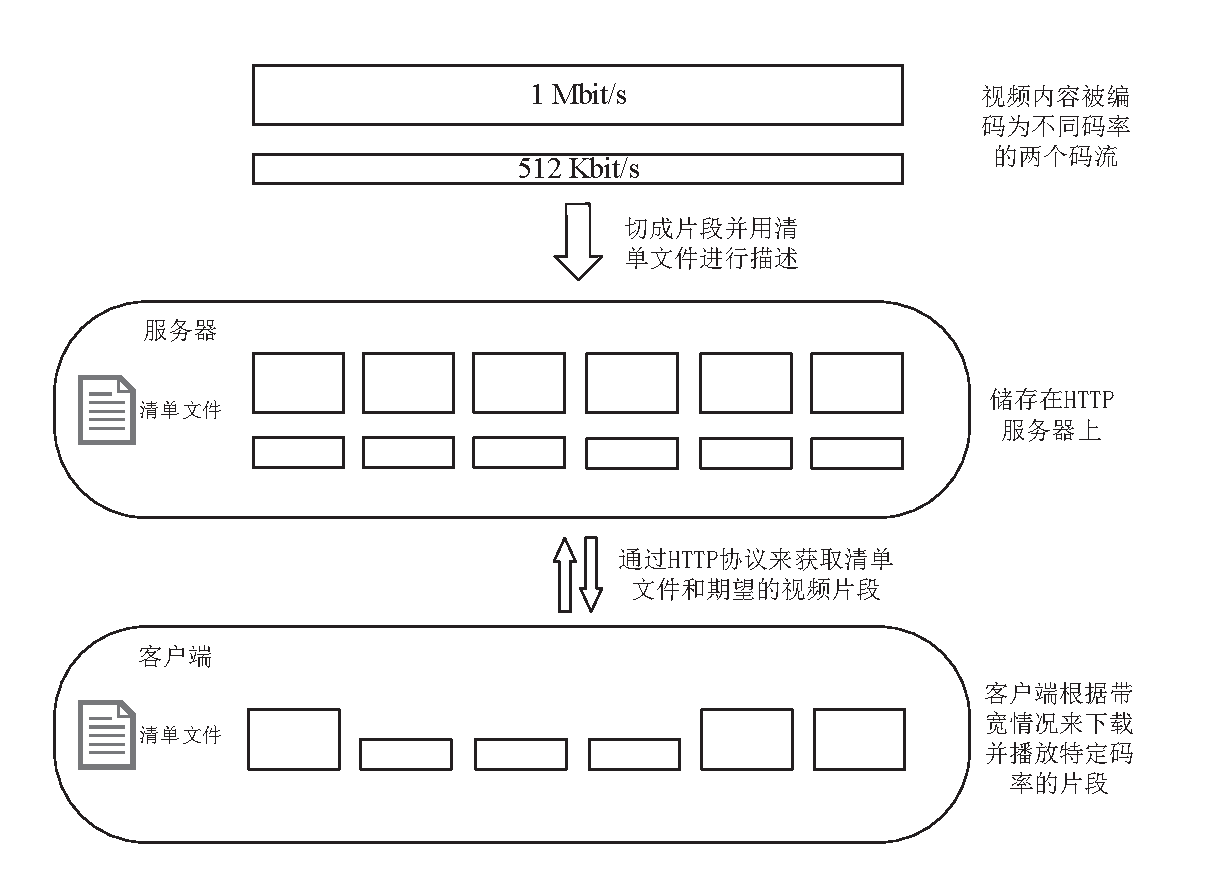
\includegraphics[width = 1.0\linewidth]{eps/DASH}
	\caption{DASH系统的工作原理示意图\label{fig:DASH}}
\end{figure}

多码流方案的优点是无需对已有的程序和系统做较大的改动,因此比较易于部署\supercite{Bouten2014}。很多商业视频网站(如YouTube、优酷等)已经用它实现了自适应功能。但是,多码流方案能提供的适应范围和粒度非常有限。例如,YouTube网站上的视频最多只提供144p、240p、360p、480p、720p和1080p这六个等级(参见图\ref{fig:youtube},其中右下角矩形框中显示了支持的等级),而优酷网上的视频大多只提供标清、高清、超清这三个画质(参见图\ref{fig:youku})。此外,多个码流的编码和存储需要大量的计算资源和磁盘空间,使得时间和空间开销成倍增加。要想以合理的代价提供精细无缝的自适应性,就需要采用可伸缩视频编码的方案。可伸缩视频码流能够以非常小的数据粒度进行码率调整,而且性能分析表明可伸缩视频编码的压缩效率远高于同一内容多次编码的多码流方法\supercite{SVC-Performance}。正是因为这些优势,基于可伸缩视频编码来实现自适应视频流媒体从技术上来说是一个更好的方案,也吸引了学术界很多研究者的关注\supercite{Chuah2012, Zhu2013, Dan2013, Yang2014, Cicalo2014}。

\begin{figure}[t]
	\centering
	\vspace{10pt}
	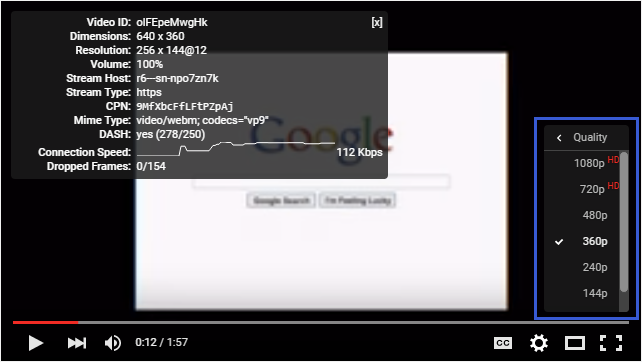
\includegraphics[width = 1.0\linewidth]{figures/youtube.png}
	\vspace{10pt}
	\caption{YouTube视频码率自适应功能图示\label{fig:youtube}}
	\vspace{10pt}
\end{figure}

\begin{figure}[t]
	\centering
	\vspace{10pt}
	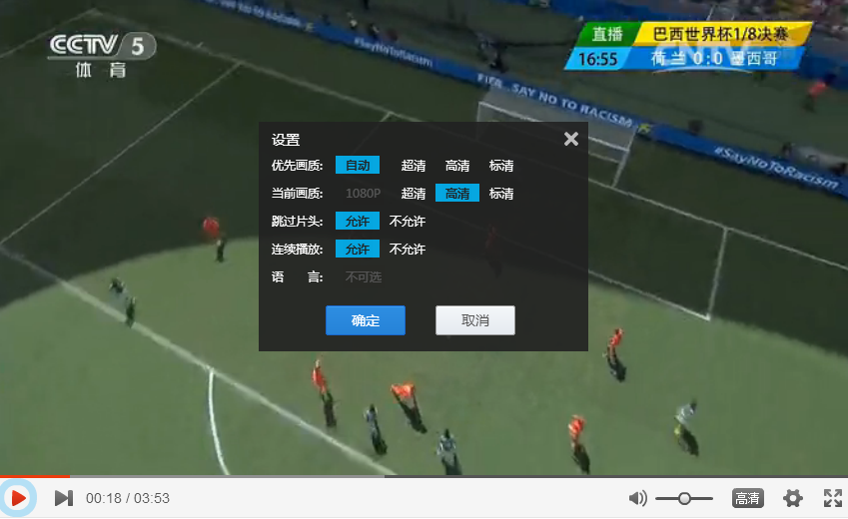
\includegraphics[width = 1.0\linewidth]{figures/youku.png}
	\vspace{10pt}
	\caption{优酷网视频码率自适应功能图示\label{fig:youku}}
	\vspace{10pt}
\end{figure}

从图\ref{fig:research-framework}所示的研究框架中可以看出,采用可伸缩视频编码或是采用DASH之类的多码流方案,其区别只在于数据源端提供可变码率的方式不同。当可伸缩视频作为数据源时,在给定码率下选择丢弃哪些数据包,即如何最优地从整个码流中截取出一个子流用于发送是需要研究的问题之一。多码流作为数据源时则不存在这个问题。而对于在传输过程中如何自动调整码率以适应带宽的变化,却是二者共有的问题。这些问题的解决,是提高视频流媒体服务质量和用户体验的关键。

\section{本文研究内容和主要贡献}

本文结合视频流媒体所面临的挑战,对自适应视频流媒体中的关键技术进行研究,以更好地解决上面所提到的问题。首先,本文针对可伸缩视频数据源提出了新的失真模型和码流截取方案,在支持可变码率的同时提供尽可能高的视频质量;其次,本文为基于可伸缩视频编码的视频点播系统设计了新的码率自动调整策略,用控制论的方法来解决如何适应带宽变化的问题;最后,本文详细分析了现在非常流行的视频直播系统的传输过程,结合直播的特点提出了数据上传时的码率自适应算法。本文主要的研究内容和创新性贡献可以归纳为如下三个部分:
\begin{enumerate}
\item {采用线性误差模型的可伸缩视频码流截取方案}\\
作为码率适应带宽波动的前提条件,视频流媒体中的数据源需要能够灵活调整。可伸缩视频编码技术通过将数据划分为基本层和增强层并丢弃增强层的数据包来实现即时码率变化。从完整的可伸缩码流中丢弃部分数据得到一个子流的过程称为码流截取。本文以最小化特定截取码率限制下的视频失真为目标,首先提出了一个线性误差模型来估计丢弃任意数据包组合带来的失真变化,然后利用它设计了一个贪心型算法来根据每个数据包的码率和失真影响对其赋优先级,作为截取过程中丢包的顺序。相比于参考软件,这一码流截取方案能够在同样的复杂度和码率限制下取得更高的视频质量。
\item {基于PID控制思想的点播系统码率自适应算法}\\
自适应视频流媒体中的另一个关键问题是传输过程中的码率调整策略,即在可用带宽不断变化的情况下,决定何时调整码率并确定调整到多少。本文基于经典的比例-积分-微分(Proportional-Integral-Derivative,PID)控制思想,提出了一个综合考虑带宽的历史状况、当前状态和未来趋势的码率自适应算法,既能充分利用带宽,传输较高的视频质量,又能减小带宽波动的影响,保证视频质量的平滑性。该算法集成在了苹果公司QuickTime流媒体服务器的开源版本上,并在实际应用中取得了很好的效果。
\item {基于缓冲区分析的直播系统码率自适应算法}\\
在视频直播中,由于数据是实时产生的,其传输过程与视频点播有所不同。视频数据需要先上传到服务器,然后由服务器分发到观看者进行播放。本文为这个过程中的上传阶段增加了码率自适应的特性:首先通过详细分析系统整个传输过程中各个缓冲区的关系,建立了一个多缓冲区模型;然后把上述点播系统中用到的PID方法与多缓冲区模型相结合,提出了一个有效的码率自适应算法。相比于没有自适应的上传过程,带宽的利用率得到了提升,视频播放的连续性也得到了改善。
\end{enumerate}

\section{本文的结构安排}

本文共分为六章,后续章节具体内容安排如下。

第二章概述自适应视频流媒体领域的研究基础和相关工作。首先对视频编码和流式传输的基础知识进行简要介绍,然后对本文所要研究的可伸缩视频码流截取、传输中的码率自适应这两个问题进行具体描述,并对已有的相关工作进行分析。

第三章讨论采用线性误差模型的码流截取方案。首先针对可伸缩视频推导并验证线性误差模型,然后介绍采用该模型的失真估计方法和以码率失真影响为度量标准的优先级赋值算法。最后展现并分析所提出的码流截取方案的实验结果。

第四章讨论基于PID控制思想的点播系统码率自适应算法。首先对PID控制器做简单的介绍,然后将PID模型运用到视频传输中的码率调整策略,提出了一个新颖的码率自适应算法。该算法被集成在了苹果公司QuickTime流媒体服务器的开源版本中,其有效性通过对比实验得到了验证。

第五章讨论针对直播系统的码率自适应算法。首先详细分析了直播系统的传输过程,提出了一个多缓冲区模型;然后将其与PID控制方法相结合,用缓冲区状态作为系统变量进行控制,实现了上传过程的码率自适应,改善了带宽利用率和视频播放的连续性。

第六章总结全文内容并对未来工作和应用前景进行展望。